% !TeX root = ../master.tex

\lecture{2}{2026-09-01}{Conduction, Pt. I}

\section{Conduction}
Heat transfer has both a \textit{direction} and a \textit{magnitude} and is therefore a vector quantity.
The magnitude in a specified direction is proportional to the \textit{temperature gradient}.
Heat conduction in a medium is \textit{steady}, when the temperature $T = T(x,y,z)$ does not vary with time and \textit{unsteady} or \textit{transient} when $T =(x,y,z,t)$ varies with time.
During transient heat transfer, the temperature normally varies with time as well as position.
In the special case of variation with time but not with position, the temperature of the medium changes uniformly with time -- such systems are termed \textit{lumped systems}.
Many small objects can be analyzed as being lumped systems.

In \Cref{sec:condintroduction}, heat conduction was defined as the transfer of thermal energy from more energetic particles of a medium to the adjacent less energetic ones.
We generally employ a coordinate system such that heat transfer in the positive direction of a coordinate axis is positive and vice versa.

We previously introduced Fourier's law of heat conduction in \Mref{eq:fourierlawconduction},
\begin{equation*}
  \dot{Q}_{\text{cond}} = -kA \frac{\mathrm{d}T}{\mathrm{d}x} 
\end{equation*}
where $k$ is the \textit{thermal conductivity} and $\frac{\mathrm{d}T}{\mathrm{d}x} $ is the temperature gradient.
In general the thermal conductivity of a material $k$ varies with time, however for most purposes an average value can be used for sufficiently accurate results.

Heat may also be generated throughout a medium.
E.g. the temperature of a resistor rises volumetrically when a current is applied.
Often it is also convenient to model the absorption of radiation such as solar energy or gamma rays as heat generation when those rays penetrate deep into a medium while being absorbed gradually such as for solar rays in a body of water.
For opaque bodies almost all absorption occurs within the first few microns of the surface, so in these cases the solar energy can be treated as heat flux on the surface. 
As heat generation is volumetric, it is usually specified per unit volume and denoted by $\dot{e}_{\text{gen}} = \left[ \unit{\W\per\m\cubed} \right]$.
The rate of heat generation may very with time as well as position.
When the variation w.r.t. the position is known, the total rate of heat generation in a medium of volume $\mathscr{V}$ can be determined from
\begin{equation} \label{eq:heatgenint}
  \dot{E}_{\text{gen}} = \int_{\mathscr{V}} \dot{e}_{\text{gen}} \, \mathrm{d}\mathscr{V}
.\end{equation}
In the special case of uniform heat generation \Mref{eq:heatgenint} reduces to
\begin{equation*}
  \dot{E}_{\text{gen}} = \dot{e}_{\text{gen}} \mathscr{V}
.\end{equation*}


\subsection{Heat Conduction Equation}
It is useful to expand \Mref{eq:fourierlawconduction} to more dimensions and include the internal heat generation.
In rectangular coordinates it can be shown that \Mref{eq:fourierlawconduction} can be written as
\begin{equation} \label{eq:heatcondcart}
  \frac{\partial }{\partial x} \left( k \frac{\partial T}{\partial x}  \right) + \frac{\partial }{\partial y} \left( k \frac{\partial T}{\partial y}  \right) + \frac{\partial }{\partial z} \left( k \frac{\partial T}{\partial z}  \right) + \dot{e}_{\text{gen}} = \rho c \frac{\partial T}{\partial t} 
.\end{equation}
for density $\rho$ and specific heat $c$.
In cylindrical coordinates it can be written
\begin{equation*}
  \frac{1}{r} \frac{\partial }{\partial r} \left( k r \frac{\partial T}{\partial r}  \right) + \frac{1}{r^2} \frac{\partial }{\partial \phi}  \left( k \frac{\partial T}{\partial \phi}  \right) + \frac{\partial }{\partial z} \left( k \frac{\partial T}{\partial z}  \right) + \dot{e}_{\text{gen}} = \rho c \frac{\partial T}{\partial t}
\end{equation*}
and in spherical coordinates it is
\begin{equation*}
  \frac{1}{r^2} \frac{\partial }{\partial r} \left( kr^2 \frac{\partial T}{\partial r}  \right) + \frac{1}{r^2 \sin^2 \theta} \frac{\partial }{\partial \phi} \left( k  \frac{\partial T}{\partial \phi} \right) + \frac{1}{r^2 \sin^2 \theta}\frac{\partial }{\partial \theta} \left( k \sin \theta \frac{\partial T}{\partial \theta}  \right) + \dot{e}_{\text{gen}} = \rho c \frac{\partial T}{\partial t} 
.\end{equation*}

\Mref{eq:heatcondcart} is the general heat conduction equation in rectangular coordinates.
In the case of constant thermal conductivity it reduces to:
\begin{equation} \label{eq:fourierbiot}
  \frac{\partial ^2 T}{\partial x^2}  + \frac{\partial ^2 T}{\partial y^2} + \frac{\partial ^2 T}{\partial z^2} + \frac{\dot{e}_{\text{gen}}}{k} = \nabla^2 T + \frac{\dot{e}_{\text{gen}}}{k} = \frac{1}{\alpha} \frac{\partial T}{\partial t}
\end{equation}
where $\alpha = k / \rho c$ is the \textit{thermal diffusivity of the material}.
\Mref{eq:fourierbiot} is known as the Fourier-Biot Equation.


\subsubsection{Special Cases of the Heat Equation}
For steady state systems the temperature does not vary with time $\frac{\partial T}{\partial t}  = 0$, so for steady-state:
\begin{equation} \label{eq:poisson}
  \frac{\partial ^2 T}{\partial x^2} + \frac{\partial ^2 T}{\partial y^2}  + \frac{\partial ^2 T}{\partial z^2} + \frac{\dot{e}_{\text{gen}}}{k} = \nabla^2 T + \frac{\dot{e}_{\text{gen}}}{k} = 0 
.\end{equation}
\Mref{eq:poisson} is known as the Poisson equation.

For transient systems with no heat generation \Mref{eq:fourierbiot} reduces to:
\begin{equation} \label{eq:diffusion}
  \frac{\partial ^2 T}{\partial x^2} + \frac{\partial ^2 T}{\partial y^2}  + \frac{\partial ^2 T}{\partial z^2} = \nabla^2 T = \frac{1}{\alpha} \frac{\partial T}{\partial t}
.\end{equation}
\Mref{eq:diffusion} is also known as the diffusion equation.

For steady-state systems without heat generation we arrive at \Mref{eq:laplace} also known as the Laplace equation:
\begin{equation*} \label{eq:laplace}
  \frac{\partial ^2 T}{\partial x^2}  + \frac{\partial ^2 T}{\partial y^2}  + \frac{\partial ^2 T}{\partial z^2} = \nabla ^2 T = 0
.\end{equation*}


\subsection{One-Dimensional Steady Heat Conduction}
We consider heat conduction through a large plane wall such as the wall of a house, the glass of a single pane window, or many other cases.
Heat conduction in these conditions can be approximated as being \textit{one-dimensional} since the conduction is dominant in one direction and negligible in the others.

\subsubsection{Plane Walls} \label{sec:planewall}
We consider a thin element of thickness $\Delta x$ in a large plane wall, as shown in \Mref{fig:condvolelement}.
We assume the density of the wall to be $\rho$, the specific heat to be $c$ and the area of
the wall normal to the direction of heat transfer to be $A$.

\begin{figure} [ht]
  \centering
  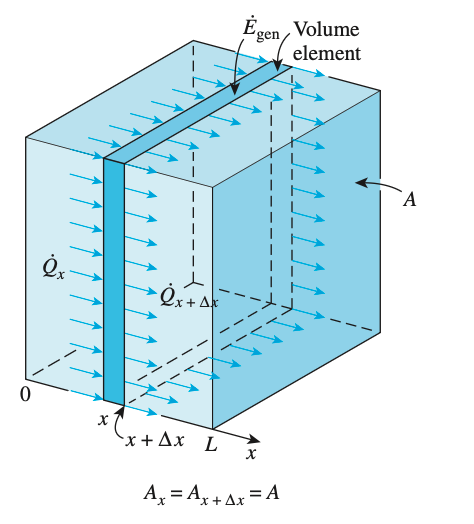
\includegraphics[width=0.5\linewidth]{./figures/condvolelement.png}
  \caption{One-dimensional heat conduction through a volume element in a large plane wall. Reproduced from \citepage{cengel2015heatmasstransfer}{fig 2--12}.}
  \label{fig:condvolelement}
\end{figure}

Taking the direction normal to the surface of the wall, i.e. through the plane on \Mref{fig:condvolelement} to be the $x$-direction we obtain:
\begin{align*}
  \frac{\mathrm{d}^2 T}{\mathrm{d}x^2} &= 0 \\
  \frac{\mathrm{d}T}{\mathrm{d}x} &= C_1 \\
  T &= C_1 x + C_2
.\end{align*}
On one side of the wall the temperature $T(0) = T_1$ and expressing the thickness of the wall as $L$ the boundary condition on the other side of the wall is $T(L) = T_2$ as shown on \Mref{fig:cond1dwall}

\begin{figure} [ht]
  \centering
  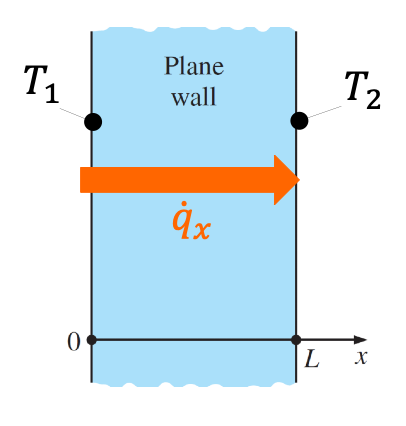
\includegraphics[width=0.6\linewidth]{./figures/cond1dwall.png}
  \caption{Conduction through a 1D-wall.}
  \label{fig:cond1dwall}
\end{figure}

As such
\begin{equation*}
  T(x) = T_1 + (T_2 - T_1) \frac{x}{L}
.\end{equation*}
This can then be used in \Mref{eq:fourierlawconduction} as
\begin{align*}
  \dot{q}_x &= -k \frac{\mathrm{d}T}{\mathrm{d}x}  \\
  \dot{q}_x(x) = \text{const.} &= k \frac{T_1 - T_2}{L} \\
  \dot{Q} &= k \frac{T_1 - T_2}{L}A 
.\end{align*}

\subsubsection{Cylindrical Geometries} \label{sec:cylgeo}
We consider a pipe of length $L$, inner and outer radiusses $r_1$ and $r_2$ and thermal conductivity $k$ as shown on \Mref{fig:f250}.

\begin{figure} [ht]
  \centering
  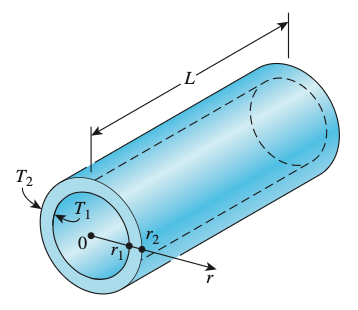
\includegraphics[width=0.5\linewidth]{./figures/f250.png}
  \caption{Schematic of a long cylinder with thickness $\Delta r = r_2 - r_1$. Reproduced from \citepage{cengel2015heatmasstransfer}{fig. 2--50}.}
  \label{fig:f250}
\end{figure}

The governing differential equation in this case is
\begin{equation*}
  \frac{\mathrm{d}}{\mathrm{d}r} \left( r \frac{\mathrm{d}T}{\mathrm{d}r}  \right) = 0 
\end{equation*}
with boundary conditions $T(r_1) = T_1, T(r_2) = T_2$.
Integrating the differential equation with respect to $r$ gives
\begin{gather*}
  r \frac{\mathrm{d}T}{\mathrm{d}r} = C_1  \frac{\mathrm{d}T}{\mathrm{d}r} = \frac{C_1}{r} \\
     T(r) = C_1 \ln r + C_2 
.\end{gather*}
Applying the boundary conditions this becomes
\begin{equation*}
  T(r) = T_1 + \left( T_2 - T_1 \right) \frac{\ln (r / r_1)}{\ln (r_2 / r_1)}
.\end{equation*}
This can be used in \Mref{eq:fourierlawconduction} as
\begin{gather*}
  \dot{q}_r (r) = -k \frac{\mathrm{d}T}{\mathrm{d}r} = k \frac{T_1-T_2}{\ln (r_2 /r_1) r} \\
  \dot{Q} = 2 \pi l k \frac{T_1 - T_2}{\ln (r_2 / r_1)}
.\end{gather*}


\subsubsection{Internal Heat Generation}
We now consider a long cylinder/wire which generates heat uniformly as shown on \Mref{fig:uniforminternalheatcyl}.
From steady state on cylindrical coordinates with uniform internal heat generatio we have
\begin{align*}
  \frac{1}{r}\frac{\mathrm{d}}{\mathrm{d}r} \left( r \frac{\mathrm{d}T}{\mathrm{d}r}  \right) + \frac{\dot{e}_{\text{gen}}}{k} &= 0 \\
  \frac{\mathrm{d}}{\mathrm{d}r} \left( r \frac{\mathrm{d}T}{\mathrm{d}r}  \right) &= - \frac{\dot{e}_{\text{gen}}}{k}r \\
  r \frac{\mathrm{d}T}{\mathrm{d}r} &= - \frac{\dot{e}_{\text{gen}}}{k} \frac{r^2}{2} + C_1 
.\end{align*}

\begin{figure} [ht]
  \centering
  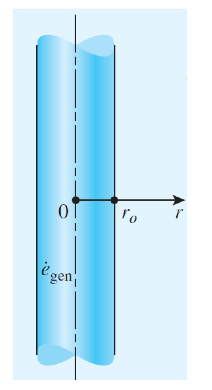
\includegraphics[width=0.3\linewidth]{./figures/uniforminternalheatcyl.png}
  \caption{Cylinder/wire conducting heat with uniform internal heat generation.}
  \label{fig:uniforminternalheatcyl}
\end{figure}

Due to symmetry we have a boundary condition at $r = 0$ as
\begin{align*}
  \frac{\mathrm{d}T}{\mathrm{d}r} (r=0) &= 0 \qquad \implies \qquad C_1 = 0 \\
  \frac{\mathrm{d}T}{\mathrm{d}r} &= - \frac{\dot{e}_{\text{gen}}}{k} \frac{r}{2} \\
  T &= - \frac{\dot{e}_{\text{gen}}}{k} \frac{r^2}{4} + C_2
.\end{align*}
Our second boundary condition is that the temperature at the edge is the surface temperature $T(r_0) = T_s$.
Hence
\begin{align*}
  T &= T_s + \frac{\dot{e}_{\text{gen}}}{4k} \left( r_0^2 - r^2 \right) \\
  T(r = 0) &= T_s + \frac{\dot{e}_{\text{gen}}}{4k} r_0^2
.\end{align*}

\subsection{Boundary Conditions}
A few different types of boundary conditions are normally employed
\begin{enumerate}
  \item Specified Temperature (Dirichlet)
  \item Specified heat flux (Neumann)
  \item Insulated boundary -- special case of Neumann with $\dot{q}_0 = 0$
  \item Thermal symmetry -- Symmetric temperature profile
  \item Convection (Robin / mixed) -- Specified convection from surfaces
\end{enumerate}

\subsection{Thermal Resistance}
Under steady conditions and surface temperatures the cumbersome differential equations can be avoided by instead introducing the concept of \textit{thermal resistivity} analogous to electrical resistivity.

\subsubsection{Conduction Resistance}
Analogous to electrical resistance:
\begin{equation*}
  I = \frac{V_1 - V_2}{R_e}
\end{equation*}
we now introduce thermal resistance
\begin{equation*}
  \dot{Q} = \frac{T_1 - T_2}{R}
.\end{equation*}
From the result for the conduction through a plane wall in \Mref{sec:planewall}
\begin{equation*}
  \dot{Q} = k \frac{T_1 - T_2}{L}A
\end{equation*}
the thermal resistivity can by comparison with the definition be read to equal
\begin{equation*}
  R_{\text{cond, wall}} = \frac{L}{kA}
.\end{equation*}
From the result for the conduction through a cylinder from \Mref{sec:cylgeo}
\begin{equation*}
  \dot{Q} = 2 \pi l k \frac{T_1 - T_2}{\ln (r_2/r_1)}
\end{equation*}
we see that the thermal resistivity here is
\begin{equation*}
  R_{\text{cond,cyl}} = \frac{\ln (r_2/r_1)}{2\pi l k}
.\end{equation*}

\subsubsection{Series Resistance Networks}
The above conduction resistances can be combined.
Say two walls are placed against each other.
Following the above the thermal conduction through each wall is
\begin{align*}
  \dot{Q}_{2} &= \frac{T_1 - T_2}{R_{\text{wall},1}} \\
  \dot{Q}_3 &= \frac{T_2 - T_3}{R_{\text{wall},2}}
.\end{align*}
We can then eliminate the intermediate temperature at the interface between the walls $T_2$ as
\begin{equation*}
  \dot{Q}_{23} = \frac{T_1 - T_3}{R_{\text{wall},1} + R_{\text{wall},2}}
.\end{equation*}
We define the convective thermal resistance as
\begin{equation*}
  \dot{Q} = h A \left( T_{\infty} - T_s \right)
.\end{equation*}
And as such for the case shown on \Mref{fig:seriesthermalres}
\begin{align*}
  \dot{Q}_{1} &= h_1 A \left( T_{\infty 1} - T_1 \right) = \frac{T_{\infty1} - T_1}{R_{\text{conv},1}}  \\
  \dot{Q}_{4} &= h_2 A \left( T_3 - T_{\infty 2} \right) = \frac{T_3 - T_{\infty 2}}{R_{\text{conv}, 2}}
.\end{align*}
These can then all be combined to yield the total conduction through the wall
\begin{equation*}
  \dot{Q} = \frac{T_{\infty 1} - T_{\infty 2}}{R_{\text{conv},1} + R_{\text{conv},2} + R_{\text{wall},1} + R_{\text{wall},2}}
.\end{equation*}


\begin{figure} [ht]
  \centering
  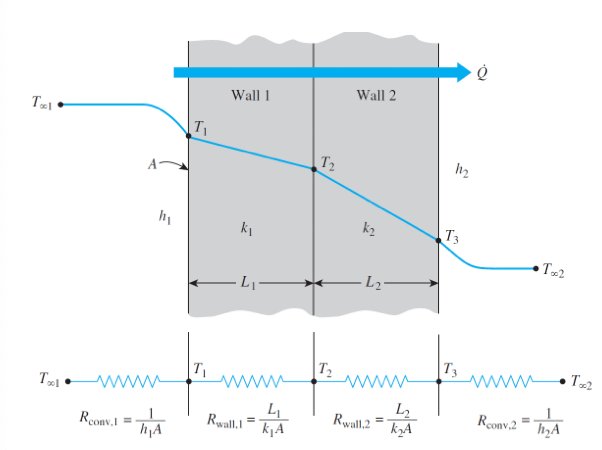
\includegraphics[width=0.7\linewidth]{./figures/seriesthermalres.png}
  \caption{Thermal resistance in series.}
  \label{fig:seriesthermalres}
\end{figure}

\subsubsection{Parallel and Generalized Resistance Networks}
Analogous to electrical resistances thermal resistances can also be in parallel as shown on \Mref{fig:parprob}.
In such cases the total resistance, $R_{\text{tot}}$ is calculated using the reciprocal of the reciprocal sums of the individual parallel resistances.
\begin{equation*}
  \frac{1}{R_{\text{tot}}} = \frac{1}{R_1} + \frac{1}{R_2}
.\end{equation*}

Parallel thermal resistances only occur in 2D or 3D whilst thermal resistance theory is based on 1D solutions so this is only an approximation.

\begin{figure} [ht]
  \centering
  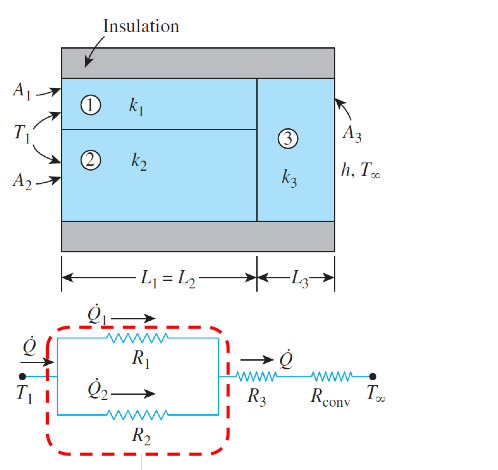
\includegraphics[width=0.5\linewidth]{./figures/parprob.png}
  \caption{Parallel thermal resistance}
  \label{fig:parprob}
\end{figure}

\subsubsection{Thermal Contact Resistance}
In the above, we assumed ``perfect contact'' at the interface between layers, and thus no temperature drop at the interface.
In reality no such interface exists and as a result any interface will contain imperfections and air gaps.
Thus, an interface offers some resistance to heat transfer which is characterised by a \textit{thermal contact resistance} $R_c$ for a unit interface area.
This can be expressed in a manner analogous to Newton's law of cooling
\begin{equation*}
  \dot{Q} = h_c A \Delta T_{\text{interface}}
\end{equation*}
where $A$ is the apparent interface area, $\Delta T_{\text{interface}}$ is the effective temperature difference at the interface and $h_c$ is the \textit{thermal contact conductance} defined as
\begin{equation*}
  h_c = \frac{\dot{Q}/A}{\Delta T_{\text{interface}}}
\end{equation*}
which is the inverse of thermal contact resistance $R_c$
\begin{equation*}
  R_c = \frac{1}{h_c} = \frac{\Delta T_{\text{interface}}}{\dot{Q}/A}
.\end{equation*}

It is also worth noting that the heat transfer rate is the quotient of the temperature difference over the interface $\Delta T_{\text{interface}}$ and the created thermal resistance $R_c / A$ as
\begin{equation*}
  \dot{Q} = \frac{\Delta T_{\text{interface}}}{R_c / A}
.\end{equation*}

